%% The first command in your LaTeX source must be the \documentclass command.
%%
%% Options:
%% twocolumn : Two column layout.
%% hf: enable header and footer.
\documentclass[
% twocolumn,
% hf,
]{ceurart}

%%
%% One can fix some overfulls
\sloppy

%%
%% Minted listings support 
%% Need pygment <http://pygments.org/> <http://pypi.python.org/pypi/Pygments>
\usepackage{listings}
%% auto break lines
\lstset{breaklines=true}

%%
%% end of the preamble, start of the body of the document source.
\begin{document}

%%
%% Rights management information.
%% CC-BY is default license.
\copyrightyear{2024}
\copyrightclause{Copyright for this paper by its authors.
  Use permitted under Creative Commons License Attribution 4.0
  International (CC BY 4.0).}

%%
%% This command is for the conference information
\conference{Alberto Mendelzon International Workshop on Foundations of Data Management}

%%
%% The "title" command
\title{Opportunities for Shape-based Optimization of Link Traversal Query Execution over Decentralized Environments}


%%
%% The "author" command and its associated commands are used to define
%% the authors and their affiliations.
\author[1]{Bryan-Elliott Tam}[%
]

\author[1]{Ruben Taelman}[%
]
\author[1]{Pieter Colpaert}[%
]


\address[1]{IDLab,
Department of Electronics and Information Systems, Ghent University – imec}

%%
%% Keywords. The author(s) should pick words that accurately describe
%% the work being presented. Separate the keywords with commas.
\begin{keywords}
  Linked data \sep
  Link Traversal Query Processing \sep
  Query containment \sep
  RDF shape \sep
  Descentralized environments \sep
  Query optimization
\end{keywords}

%%
%% This command processes the author and affiliation and title
%% information and builds the first part of the formatted document.
\maketitle


\begin{abstract}
    % Context
    Linked Data on the Web can be considered as one very large Decentralized Knowledge Graph.
    % Need
    While centralized query processing approaches are well-understood,
    decentralization-friendly alternatives with no prior index such as Link Traversal Query Processing (LTQP)
    are insufficiently performant for real-world use cases.
    Indeed, LTQP approaches on the web are difficult due to the pseudo-infinite size of the domain,
    the unstructured nature of the medium,
    and the lack of a priori information for query planning.
    For most traversal-based queries the execution of a large number of HTTP requests is the bottleneck. 
    However, in practice, queries target small subsets of the Web.
    Web subsets are always structured either implicitly or explicitly.
    Explicit structure can be described via hypermedia descriptions.
    Using those structural information query engines can improve
    their performances by reducing their search domain.
    % Task
    Our goal is to explore the opportunities of using mappings between RDF data shapes and distributed RDF subgraphs
    for the purpose of improving the performance of traversal-based queries.
    % Object
    In this article, we discuss these opportunities, present preliminary results, and discuss potential future work.
    % Findings
    Our initial experiments show that with little maintenance and work from the server,
    our method can significantly reduce the number of links traversed to answer a query leading to
    a substantial reduction in query execution time compared to the state of the art.
    % Perspectives
    In future work, we are going to formalize our method, perform more extensive experiments,
    and design algorithms for query planning that take into consideration this shape metadata.
    
    
\end{abstract}
\section{Introduction}

\sepfootnotecontent{fn:typeIndex}{
  \href{https://solid.github.io/type-indexes/}{https://solid.github.io/type-indexes/}
}

The World Wide Web is a naturally decentralized database.
Centralizing large web segments in single endpoints provides easier query interfaces and faster query execution times.
However, data centralization can lead to practices that raise ethical and legal concerns, making the exploration of decentralization-friendly query paradigms a relevant research topic.
The query languages webSQL~\cite{Mendelzon1996} and \href{https://www.w3.org/TR/sparql11-query/}{SPARQL} propose mechanisms to capture decentralized web data with conjunctive queries.
However, webSQL relies on web indexing~\cite{Mendelzon1996}.
Indexing processes can be expensive, particularly on the scale of the web, and necessitate frequent updates, furthermore, they can be restrictive by excluding some sources thus hindering the natural serendipity of the web.
SPARQL solutions rely on the publication of linked data.
Linked data in their structure particularly with the presence of IRI gives the opportunity to find more related information without indexes.
However, most query processing over linked data is performed in centralized and federated setups, leaving indexing-independent approaches largely experimental.

Link Traversal Query Processing (LTQP)~\cite{Hartig2012} is a method to query unindexed networks of linked data documents.
The method consists of starting from an initial set of IRIs concurrently answer the query provided by the user while dereferencing IRIs leading to external data sources from the internal engine triple store.
While LTQP enables live exploration of environments without prior indexing, it leads to some difficulties.
One of them is the pseudo-infinite search domain derived from the size of the World Wide Web~\cite{hartig2016walking}.
Additionally, HTTP requests can be very slow and unpredictable making their execution the bottleneck of the method~\cite{hartig2016walking}.
Reachability criteria~\cite{Hartig2012} are a partial answer to this problem by defining completeness based on the traversal of URIs
contained in the internal data source of the engine instead of on the acquisition of all the results or the traversal of the whole web.
Another difficulty is the lack of a priori information about the sources rendering query planning challenging.
To alleviate this problem, the current state-of-the-art consists of using carefully crafted heuristics for joins ordering~\cite{Hartig2011}.
The limitations of the heuristics approach are usually of little importance because the main bottleneck is the high number of HTTP requests.

Earlier LTQP research has focused on the open web.
More recently, LTQP research has shifted its focus to environments where the structure of data publication provides useful information for query optimization.
This line of research uses \emph{structural assumptions}~\cite{Taelman2023} to guide query engines~\cite{verborgh2020guided} towards relevant data sources.
Structural assumptions act as contracts between the data provider and the query engines stipulating that within a certain subdomain of the web, information meeting a specific constraint can be found.
The use of structural assumptions has been studied in Solid \cite{Taelman2023}.
The method involves the utilization of the 
\href{https://solidproject.org/TR/protocol#resources}{solid storage} hypermedia description~\cite{Fielding} to locate all the resources of a pod. 
This hypermedia description is not expressive enough to capture the content of the resources of a pod, thus, for query-aware optimizations, the \href{https://solid.github.io/type-indexes/}{type index specification}~\sepfootnote{fn:typeIndex} is additionally used.
The type index formulation proposes a more declarative approach~\cite{Taelman2017} by mapping RDF classes with sets of resources.
By using those structural assumptions it is possible to reduce the query execution time of realistic queries to the extent where the bottleneck is not the execution of HTTP requests but the suboptimal heuristic-based query plan~\cite{eschauzier_quweda_2023, Taelman2023}.
Yet, for multiple queries the high number of HTTP requests remains the main bottleneck~\cite{eschauzier_quweda_2023}.
It is reasonable to hypothesize that a significant portion of those HTTP requests lead to the dereferencing of documents containing data that do not contribute to the result of the query.
Hence, investigating more descriptive structural assumptions is a relevant research endeavor.

In this article, we propose to use RDF data shapes as the main mechanism for a structural assumption in the form of a shape index.
RDF data shapes are mostly used in data validation~\cite{Gayo2018a} thus, they provided a good formalization to describe the structure of data.
Additionally, to a lesser extent, they have been used for query optimizations~\cite{kashif2021}.
The shape index is an early effort for data summarisation of decentralized datasets~\cite{Stuckenschmidt2004,Goldman1997, Harth2010} within networks of unindexed linked data documents.
The current focus of the index is source selection.
However, we foresee opportunities to use a similar approach for link queue ordering and query planning.
This paper presents our preliminary work on data discovery and link pruning thus tackling the problem of the large search space of LTQP queries in linked data environments with structure.

\section{Shape index and query-shape containment}

We define a shape index as a set of mappings between RDF data shapes and sets of resources.
Additionally, an SI has an associated domain (set of URLs)
and a flag indicating if the SI is \emph{complete}.
A SI is complete when every resource in the domain is associated with a shape.
In a SI when a shape is in relation to a set of RDF resources then the shape must validate them.
Furthermore, every set of triples respecting the shape in the domain must be located inside one resource of the set.

Our approach consists of determining before the traversal of a whole domain the location of the useful resources for the query execution.
This data discovery operation results in the implicit pruning of links leading to surely non-contributing resources.
In this approach, the query engine can start its processing with a permissive reachability criteria
such as $c_{all}$ \cite{Hartig2012} or the Solid state of the art reachability criterion ($c_{LDP}$ and $c_{\text{type index}}$) \cite{Taelman2023}
and not suffer the associated longer execution time during the traversal of environments containing a SI.
Indeed, after the analysis of the SI with the query provided by the user the criteria can be adapted to become more restrictive within the domain of the SI.
For that purpose, the query engine must first discover the SI in the current (sub)domain.
In the case of Solid, the SI should be at the root of the pod to be easily discoverable.
The approach is schematized at Figure \ref{fig:shape_index}.
Source selection with an SI consists of interpreting the binding results from a \emph{query-shape containment} problem similar to the classic query containment problem \cite{afariQCE, Spasi2023}.
To perform this algorithm, we propose that we can transform a shape into a query ($Q_{s}$).
In this short paper, we don't provide proof for this proposition, however, 
\citeauthor{Delva2021} give an intuition by demonstrating how to query RDF subgraphs using RDF data shapes as a query language.
The algorithm divides the query into multiple star patterns with their dependencies ($Q_{star}$).
Then it pushdown \cite{Yang2021FlexPushdownDBHP} the (sub)queries to the level of source selection to evaluate if the $Q_{star}$ are contained inside the $Q_s$ of the SI.
If all the $Q_{star}$ are contained in a $Q_{s}$ or have no binding with any $Q_{s}$
the reachability criteria is adapted to ignore all the resources not linked to a $Q_{s}$ even if the SI is \emph{incomplete}.
If the SI is \emph{complete} and not all the $Q_{star}$ are contained in a $Q_{s}$ the reachability criteria can be adapted
to visit every resource in relation to a $Q_{s}$ with a partial binding with a $Q_{star}$.
In a similar case with a \emph{incomplete} SI the query engine can only uses the SI for data discovery.
This is similar to the usage of the type index but with a larger direct reach because the properties are described in the shapes
whereas with the type index, the engine can either directly match queries describing the class of its star patterns or perform
another dereferencing operation to the class described in the index and then match the properties of the class with those defined in the star patterns \cite{Taelman2023}.

\begin{figure}
    \centering
    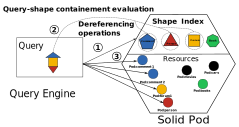
\includegraphics[width=0.5\textwidth]{figure/shape_containement}
    \caption{A schema of the source selection algorithm with a SI. First, the SI is dereference, 
    then the \emph{query-shape containment} is performed lastly only the relevant resources are dereferenced.}
    \label{fig:shape_index}
\end{figure}
\section{Preliminary results}

\begin{figure}[!h]
    \centering
    \includesvg[width=0.8\linewidth]{figure/combined}
    \caption{The query execution time distribution (the upper graph) and the number of HTTP requests (the lower graph).
    The results of our approach are in blue and the state of the art (type index with LDP) in red.
    The results have been generated with 50 repetitions and a timeout of 6000 ms. 
    The queries are denoted with first the initial of the query template (e.g., S1 for interactive-\textbf{s}hort-\textbf{1}), and the version
     of the concrete query (e.g., V0). 
     Values not present in the plot indicate that the query timeout before the end of the execution.
    }
    \label{fig:result}
\end{figure}

\sepfootnotecontent{impl}{Available at the following link \newline
\href{https://github.com/constraintAutomaton/comunica-feature-link-traversal/tree/feature/shapeIndex}{https://github.com/constraintAutomaton/comunica-feature-link-traversal/tree/feature/shapeIndex}.}

\sepfootnotecontent{benchmark}{We executed interactive-short 1 and 5, interactive-discover 1,3-7 and interactive-complex 8 with
a modified benchmark containing a \href{https://github.com/constraintAutomaton/rdf-dataset-fragmenter.js/tree/feature/shapeIndex}{\emph{complete} shape index}.
The implementation of the benchmark and complementary results are available at the following link 
\href{https://github.com/constraintAutomaton/amw_shape_index_results}{https://github.com/constraintAutomaton/amw\_shape\_index\_results}.}

For early evaluation, we implemented the containment algorithm described in the previous section.
An open implementation of the \href{https://github.com/constraintAutomaton/query-shape-detection}{algorithm} and an \href{https://github.com/constraintAutomaton/comunica-feature-link-traversal/tree/feature/shapeIndex}{integration} in the query engine Comunica \cite{taelman_iswc_resources_comunica_2018} is available online \sepfootnote{impl}.
In its current state, the implementation doesn't support 
\href{https://www.w3.org/TR/sparql11-query/#propertypaths}{SPARQL property paths} and nested queries.
We use the benchmark Solidbench \cite{Taelman2023} to compare our approach with the current state of the art 
(a combination of the type index and the \href{https://www.w3.org/TR/ldp/}{LDP specification} as structural assumptions) \cite{Taelman2023}.
To accommodate the limitation of our implementation we use a subset of the queries of Solidbench.
The benchmark with complementary results is open source and available online \sepfootnote{benchmark}.
We executed each query 50 times with a timeout of 1 minute (6,000 ms).
The results are presented in Figure \ref{fig:result}.
In Figure \ref{fig:result}, we notice that in the best-case scenario, the percentage of the reduction can be as high as 80\% (D1V3 and S1V3) for the execution time 
and 97\% (S1V3) for the number of HTTP requests.
However, there is not a direct correlation between the reduction of execution time and HTTP requests (e.g., the ratio 
between our approach and the state of the art of the number of HTTP request by the execution time for D1V3 is 0.5 compared to 0.15 for S1V3).
This hints at the results from the state of the art \cite{Taelman2023} proposing that the query plan is the bottleneck for some queries in this environment,
however, the overhead of the containment calculation could also be a contributing factor to the current results.
Our approach reliably executes fewer HTTP requests compared to the state of the art.
This is an expected result because no queries target (implicitly) each file of a user.
In the worst cases, our approach  has similar query execution times with a 
distribution tending to be lower than the state of the art (with the exception to D3V3 and D3V4 with an augmentation of 9\% of the mean of the execution time).
Furthermore, their variances tend to be lower compared to their counterpart. 
One possible explanation is that the execution time of HTTP requests is not constant and can be unpredictable \cite{hartig2016walking}
which could lead to an increase in variance.
This observation not only has potential implications for the reliability of multiple executions in terms of execution time
but also in terms of the performance of single execution in unstable networks where the server might take longer times to respond. 

\input{section/Conclusion}

% --- Bibliography ---

\bibliography{references}

\end{document}

%%
%% End of file
